%%%%%%%%%%%%%%%%%%%%%%%%%%%%%%%%%%%%%%%%
% datoteka diploma-vzorec.tex
%
% vzorčna datoteka za pisanje diplomskega dela v formatu LaTeX
% na UL Fakulteti za računalništvo in informatiko
%
% vkup spravil Gašper Fijavž, december 2010
% 
%
%
% verzija 12. februar 2014 (besedilo teme, seznam kratic, popravki Gašper Fijavž)
% verzija 10. marec 2014 (redakcijski popravki Zoran Bosnić)
% verzija 11. marec 2014 (redakcijski popravki Gašper Fijavž)
% verzija 15. april 2014 (pdf/a 1b compliance, not really - just claiming, Damjan Cvetan, Gašper Fijavž)
% verzija 23. april 2014 (privzeto cc licenca)
% verzija 16. september 2014 (odmiki strain od roba)
% verzija 28. oktober 2014 (odstranil vpisno številko)
% verija 5. februar 2015 (Literatura v kazalu, online literatura)
% verzija 25. september 2015 (angl. naslov v izjavi o avtorstvu)
% verzija 26. februar 2016 (UL izjava o avtorstvu)
% verzija 16. april 2016 (odstranjena izjava o avtorstvu)
% verzija 5. junij 2016 (Franc Solina dodal vrstice, ki jih je označil s svojim imenom)


\documentclass[a4paper, 12pt]{book}
%\documentclass[a4paper, 12pt, draft]{book}  Nalogo preverite tudi z opcijo draft, ki vam bo pokazala, katere vrstice so predolge!



\usepackage[utf8]{inputenc}   % omogoča uporabo slovenskih črk kodiranih v formatu UTF-8
\usepackage[slovene,english]{babel}    % naloži, med drugim, slovenske delilne vzorce

%\usepackage{biblatex}
%\addbibresource{literatura.bib}

\usepackage[pdftex]{graphicx}  % omogoča vlaganje slik različnih formatov
\graphicspath{ {./images/} }

\usepackage{float}          % poskrbi, na primer, za glave strani
\usepackage{fancyhdr}          % poskrbi, na primer, za glave strani
\usepackage{amssymb}           % dodatni simboli
\usepackage{amsmath}           % eqref, npr.
\usepackage{hyperxmp}
%\usepackage[hyphens]{url}  % dodal Solina
%\usepackage{comment}       % dodal Solina
\usepackage[pdftex, colorlinks=true,
  						citecolor=black, filecolor=black, 
  						linkcolor=black, urlcolor=black,
  						pagebackref=false, 
  						pdfproducer={LaTeX}, pdfcreator={LaTeX}, hidelinks]{hyperref}
 
%\usepackage[separate-uncertainty=true,multi-part-units=repeat]{siunitx}

\usepackage{color}       % dodal Solina
\usepackage{soul}       % dodal Solina

%%%%%%%%%%%%%%%%%%%%%%%%%%%%%%%%%%%%%%%%
%	DIPLOMA INFO
%%%%%%%%%%%%%%%%%%%%%%%%%%%%%%%%%%%%%%%%
\newcommand{\ttitle}{Avtomatizacija delavniškega dnevnika}
\newcommand{\ttitleEn}{Workshop report automatisation}
\newcommand{\tsubject}{\ttitle}
\newcommand{\tsubjectEn}{\ttitleEn}
\newcommand{\tauthor}{Anej Lekše}
\newcommand{\tkeywords}{mobilni razvoj, glasovni asistenti, razpoznava glasu, informacijski sistemi}
\newcommand{\tkeywordsEn}{mobile development, voice assistants, voice recognition, information systems}


%%%%%%%%%%%%%%%%%%%%%%%%%%%%%%%%%%%%%%%%
%	HYPERREF SETUP
%%%%%%%%%%%%%%%%%%%%%%%%%%%%%%%%%%%%%%%%
\hypersetup{pdftitle={\ttitle}}
\hypersetup{pdfsubject=\ttitleEn}
\hypersetup{pdfauthor={\tauthor, al1617@student.uni-lj.si}}
\hypersetup{pdfkeywords=\tkeywordsEn}


 


%%%%%%%%%%%%%%%%%%%%%%%%%%%%%%%%%%%%%%%%
% postavitev strani
%%%%%%%%%%%%%%%%%%%%%%%%%%%%%%%%%%%%%%%%  

\addtolength{\marginparwidth}{-20pt} % robovi za tisk
\addtolength{\oddsidemargin}{40pt}
\addtolength{\evensidemargin}{-40pt}

\renewcommand{\baselinestretch}{1.3} % ustrezen razmik med vrsticami
\setlength{\headheight}{15pt}        % potreben prostor na vrhu
\renewcommand{\chaptermark}[1]%
{\markboth{\MakeUppercase{\thechapter.\ #1}}{}} \renewcommand{\sectionmark}[1]%
{\markright{\MakeUppercase{\thesection.\ #1}}} \renewcommand{\headrulewidth}{0.5pt} \renewcommand{\footrulewidth}{0pt}
\fancyhf{}
\fancyhead[LE,RO]{\sl \thepage} 
%\fancyhead[LO]{\sl \rightmark} \fancyhead[RE]{\sl \leftmark}
\fancyhead[RE]{\sc \tauthor}              % dodal Solina
\fancyhead[LO]{\sc Diplomska naloga}     % dodal Solina


\newcommand{\BibTeX}{{\sc Bib}\TeX}

%%%%%%%%%%%%%%%%%%%%%%%%%%%%%%%%%%%%%%%%
% naslovi
%%%%%%%%%%%%%%%%%%%%%%%%%%%%%%%%%%%%%%%%  


\newcommand{\autfont}{\Large}
\newcommand{\titfont}{\LARGE\bf}
\newcommand{\clearemptydoublepage}{\newpage{\pagestyle{empty}\cleardoublepage}}
\setcounter{tocdepth}{1}	      % globina kazala

%%%%%%%%%%%%%%%%%%%%%%%%%%%%%%%%%%%%%%%%
% konstrukti
%%%%%%%%%%%%%%%%%%%%%%%%%%%%%%%%%%%%%%%%  
\newtheorem{izrek}{Izrek}[chapter]
\newtheorem{trditev}{Trditev}[izrek]
\newenvironment{dokaz}{\emph{Dokaz.}\ }{\hspace{\fill}{$\Box$}}

%%%%%%%%%%%%%%%%%%%%%%%%%%%%%%%%%%%%%%%%%%%%%%%%%%%%%%%%%%%%%%%%%%%%%%%%%%%%%%%
%% PDF-A
%%%%%%%%%%%%%%%%%%%%%%%%%%%%%%%%%%%%%%%%%%%%%%%%%%%%%%%%%%%%%%%%%%%%%%%%%%%%%%%


%%%%%%%%%%%%%%%%%%%%%%%%%%%%%%%%%%%%%%%% 
% define medatata
%%%%%%%%%%%%%%%%%%%%%%%%%%%%%%%%%%%%%%%% 
\def\Title{\ttitle}
\def\Author{\tauthor, al1617@student.uni-lj.si}
\def\Subject{\ttitleEn}
\def\Keywords{\tkeywordsEn}

%%%%%%%%%%%%%%%%%%%%%%%%%%%%%%%%%%%%%%%% 
% \convertDate converts D:20080419103507+02'00' to 2008-04-19T10:35:07+02:00
%%%%%%%%%%%%%%%%%%%%%%%%%%%%%%%%%%%%%%%% 
\def\convertDate{%
    \getYear
}

{\catcode`\D=12
 \gdef\getYear D:#1#2#3#4{\edef\xYear{#1#2#3#4}\getMonth}
}
\def\getMonth#1#2{\edef\xMonth{#1#2}\getDay}
\def\getDay#1#2{\edef\xDay{#1#2}\getHour}
\def\getHour#1#2{\edef\xHour{#1#2}\getMin}
\def\getMin#1#2{\edef\xMin{#1#2}\getSec}
\def\getSec#1#2{\edef\xSec{#1#2}\getTZh}
\def\getTZh +#1#2{\edef\xTZh{#1#2}\getTZm}
\def\getTZm '#1#2'{%
    \edef\xTZm{#1#2}%
    \edef\convDate{\xYear-\xMonth-\xDay T\xHour:\xMin:\xSec+\xTZh:\xTZm}%
}

\expandafter\convertDate\pdfcreationdate 

%%%%%%%%%%%%%%%%%%%%%%%%%%%%%%%%%%%%%%%%
% get pdftex version string
%%%%%%%%%%%%%%%%%%%%%%%%%%%%%%%%%%%%%%%% 
\newcount\countA
\countA=\pdftexversion
\advance \countA by -100
\def\pdftexVersionStr{pdfTeX-1.\the\countA.\pdftexrevision}


%%%%%%%%%%%%%%%%%%%%%%%%%%%%%%%%%%%%%%%%
% XMP data
%%%%%%%%%%%%%%%%%%%%%%%%%%%%%%%%%%%%%%%%  
\usepackage{xmpincl}
\includexmp{pdfa-1b}

%%%%%%%%%%%%%%%%%%%%%%%%%%%%%%%%%%%%%%%%
% pdfInfo
%%%%%%%%%%%%%%%%%%%%%%%%%%%%%%%%%%%%%%%%  
\pdfinfo{%
    /Title    (\ttitle)
    /Author   (\tauthor, damjan@cvetan.si)
    /Subject  (\ttitleEn)
    /Keywords (\tkeywordsEn)
    /ModDate  (\pdfcreationdate)
    /Trapped  /False
}


%%%%%%%%%%%%%%%%%%%%%%%%%%%%%%%%%%%%%%%%%%%%%%%%%%%%%%%%%%%%%%%%%%%%%%%%%%%%%%%
%%%%%%%%%%%%%%%%%%%%%%%%%%%%%%%%%%%%%%%%%%%%%%%%%%%%%%%%%%%%%%%%%%%%%%%%%%%%%%%

\begin{document}
\selectlanguage{slovene}
\frontmatter
\setcounter{page}{1} %
\renewcommand{\thepage}{}       % preprecimo težave s številkami strani v kazalu
\newcommand{\sn}[1]{"`#1"'}                    % dodal Solina (slovenski narekovaji)

%%%%%%%%%%%%%%%%%%%%%%%%%%%%%%%%%%%%%%%%
%naslovnica
 \thispagestyle{empty}%
   \begin{center}
    {\large\sc Univerza v Ljubljani\\%
      Fakulteta za računalništvo in informatiko}%
    \vskip 10em%
    {\autfont \tauthor\par}%
    {\titfont \ttitle \par}%
    {\vskip 3em \textsc{DIPLOMSKO DELO\\[5mm]         % dodal Solina za ostale študijske programe
    VISOKOŠOLSKI STROKOVNI ŠTUDIJSKI PROGRAM\\ PRVE STOPNJE\\ RAČUNALNIŠTVO IN INFORMATIKA}\par}%
%    UNIVERZITETNI  ŠTUDIJSKI PROGRAM\\ PRVE STOPNJE\\ RAČUNALNIŠTVO IN INFORMATIKA}\par}%
%    INTERDISCIPLINARNI UNIVERZITETNI\\ ŠTUDIJSKI PROGRAM PRVE STOPNJE\\ RAČUNALNIŠTVO IN MATEMATIKA}\par}%
%    INTERDISCIPLINARNI UNIVERZITETNI\\ ŠTUDIJSKI PROGRAM PRVE STOPNJE\\ UPRAVNA INFORMATIKA}\par}%
%    INTERDISCIPLINARNI UNIVERZITETNI\\ ŠTUDIJSKI PROGRAM PRVE STOPNJE\\ MULTIMEDIJA}\par}%
    \vfill\null%
    {\large \textsc{Mentor}: doc.\ dr.  Andrej Brodnik\par}%
   %{\large \textsc{Somentor}:  izr.\ prof.\ dr. Martin Krpan \par}%
    {\vskip 2em \large Ljubljana, 2020 \par}%
\end{center}
% prazna stran
%\clearemptydoublepage      % dodal Solina (izjava o licencah itd. se izpiše na hrbtni strani naslovnice)

%%%%%%%%%%%%%%%%%%%%%%%%%%%%%%%%%%%%%%%%
%copyright stran
\thispagestyle{empty}
\vspace*{8cm}

\noindent
{\sc Copyright}. 
Rezultati diplomske naloge so intelektualna lastnina avtorja in Fakultete za računalništvo in informatiko Univerze v Ljubljani.
Za objavo in koriščenje rezultatov diplomske naloge je potrebno pisno privoljenje avtorja, Fakultete za računalništvo in informatiko ter mentorja.

\begin{center}
\mbox{}\vfill
\emph{Besedilo je oblikovano z urejevalnikom besedil \LaTeX.}
\end{center}
% prazna stran
\clearemptydoublepage

%%%%%%%%%%%%%%%%%%%%%%%%%%%%%%%%%%%%%%%%
% stran 3 med uvodnimi listi
\thispagestyle{empty}
\vspace*{4cm}

\noindent
Fakulteta za računalništvo in informatiko izdaja naslednjo nalogo:
\medskip
\begin{tabbing}
\hspace{32mm}\= \hspace{6cm} \= \kill




Tematika naloge:
\end{tabbing}
%Besedilo teme diplomskega dela študent prepiše iz študijskega informacijskega sistema, kamor ga je vnesel mentor. V nekaj stavkih bo opisal, kaj pričakuje od kandidatovega diplomskega dela. Kaj so cilji, kakšne metode uporabiti, morda bo zapisal tudi ključno literaturo.
Preveri ali so glasovni asistenti v trenutnem stanju primerni za pomoč pri pisanju delavniških dnevnikov.
Seznani se z obstoječimi programskimi rešitvami in jih analiziraj.
Po analizi trga se loti izdelave svojega sistema za pisanje delavniških dnevnikov, ki vključuje glasovnega asistenta.
\vspace{15mm}



\vspace{2cm}

% prazna stran
\clearemptydoublepage

% zahvala
\thispagestyle{empty}\mbox{}\vfill\null\it%
\noindent
Na tem mestu zapišite, komu se zahvaljujete za izdelavo diplomske naloge. Pazite, da ne boste koga pozabili. Utegnil vam bo zameriti. Temu se da izogniti tako, da celotno zahvalo izpustite.
\rm\normalfont

% prazna stran
\clearemptydoublepage

%%%%%%%%%%%%%%%%%%%%%%%%%%%%%%%%%%%%%%%%
% posvetilo, če sama zahvala ne zadošča :-)
\thispagestyle{empty}\mbox{}{\vskip0.20\textheight}\mbox{}\hfill\begin{minipage}{0.55\textwidth}%
%Svoji dragi Alenčici.
\normalfont\end{minipage}

% prazna stran
\clearemptydoublepage


%%%%%%%%%%%%%%%%%%%%%%%%%%%%%%%%%%%%%%%%
% kazalo
\pagestyle{empty}
\def\thepage{}% preprecimo tezave s stevilkami strani v kazalu
\tableofcontents{}


% prazna stran
\clearemptydoublepage

%%%%%%%%%%%%%%%%%%%%%%%%%%%%%%%%%%%%%%%%
% seznam kratic

\chapter*{Seznam uporabljenih kratic}  % spremenil Solina, da predolge vrstice ne gredo preko desnega roba

% \begin{comment}
% \begin{tabular}{l|l|l}
%   {\bf kratica} & {\bf angleško} & {\bf slovensko} \\ \hline
%   % after \\: \hline or \cline{col1-col2} \cline{col3-col4} ...
%   {\bf CA} & classification accuracy & klasifikacijska točnost \\
%   {\bf DBMS} & database management system & sistem za upravljanje podatkovnih baz \\
%   {\bf SVM} & support vector machine & metoda podpornih vektorjev \\
%   \dots & \dots & \dots \\
% \end{tabular}
% \end{comment}

\noindent\begin{tabular}{p{0.1\textwidth}|p{.4\textwidth}|p{.4\textwidth}}    % po potrebi razširi prvo kolono tabele na račun drugih dveh!
  {\bf kratica} & {\bf angleško}                             & {\bf slovensko} \\ \hline
  {\bf API} & Application Programming Interface & vmesnik za programiranje \\
  {\bf AWS} & Amazon Web Services & Amazonove spletne storitve \\
  {\bf LIMS} & Laboratory Information Management System & laboratorijski sistem za uporavljanje informacij \\
  {\bf MVVM} & Model View View-Model & Model Pogled Pogled-Model \\
  {\bf SNS} & Simple Notification Service & preprosta storitev za opozorila \\
  {\bf SQS} & Simple Queue Service & preprosta vrstna storitev \\
  {\bf UI} & User Interface & uporabniški vmesnik \\
  {\bf VUI} & Voice User Interface & glasovni uporabniški vmesnik \\
  {\bf XAML} & Extensible Application Markup Langugage & razširljiv aplikacijski označitveni? jezik \\
  {\bf XAML} & Extensible Application Markup Langugage & razširljiv aplikacijski označitveni? jezik \\
%  \dots & \dots & \dots \\
\end{tabular}


% prazna stran
\clearemptydoublepage

%%%%%%%%%%%%%%%%%%%%%%%%%%%%%%%%%%%%%%%%
% povzetek
\addcontentsline{toc}{chapter}{Povzetek}
\chapter*{Povzetek}

\noindent\textbf{Naslov:} \ttitle
\bigskip

\noindent\textbf{Avtor:} \tauthor
\bigskip

%\noindent\textbf{Povzetek:} 
%\noindent V vzorcu je predstavljen postopek priprave diplomskega dela z uporabo okolja \LaTeX. Vaš povzetek mora sicer vsebovati približno 100 besed, ta tukaj je odločno prekratek.se image upload pa vse mam nekje kodo od sihta
%Dober povzetek vključuje: (1) kratek opis obravnavanega problema, (2) kratek opis vašega pristopa za reševanje tega problema in (3) (najbolj uspešen) rezultat ali prispevek magistrske naloge.

\noindent Diplomsko delo obravnava področje izboljšanja procesa pisanja delavniškega dnevnika ali laboratorijskega poročila.
Največ časa anketirani študentje porabijo za prepisovanje v digitalno obliko, zapisovanje zapiskov na papir in urejanje teh zapiskov. 
Cilj je preizkusiti računalniški sistem z glasovnim asistentom, s pomočjo katerega lahko narekujemo zapiske med delom. 
Te zapiske pa lahko naknandno urejamo s pomočjo mobilne ali namizne aplikacije.
Uporabili bomo Amazon Alexo zaradi enostavne izdelave lastnih programov (t.i. Skill-ov).
%Rezultat te raziskave je bil, da so trenutne tehnike razpoznavanja govora pri glasovnemu asistentu Amazon Alexa še nezadostne za učinkovito delo.
%Načini in metode, kako lahko takšne naprave programiramo in uporabljamo v svojih informacijskih rešitvah pa so odlične in dobro dokumentirane.

\bigskip

\noindent\textbf{Ključne besede:} \tkeywords.
% prazna stran
\clearemptydoublepage

%%%%%%%%%%%%%%%%%%%%%%%%%%%%%%%%%%%%%%%%
% abstract
\selectlanguage{english}
\addcontentsline{toc}{chapter}{Abstract}
\chapter*{Abstract}

\noindent\textbf{Title:} \ttitleEn
\bigskip

\noindent\textbf{Author:} \tauthor
\bigskip

%\noindent\textbf{Abstract:} 
%\noindent This sample document presents an approach to typesetting your BSc thesis using \LaTeX. 
%A proper abstract should contain around 100 words which makes this one way too short.
\noindent This thesis deals with the process of optimising the process of writing a lab report.
Students, that took part in the survey, spend the most time to type the report into a digital format, write notes on paper and ordering their notes.
The goal of thesis is testing a system with a voice assistant that could be used to take notes during work itself.
These notes can be edited and ordered later via a mobile or desktop application.
We will use Amazon Alexa as it offers simple programming with Alexa Skills.
%As a result of this research, I found out that techniques of voice recognition with Amazon Alexa voice assistant were inadequate for fluent and efficient work.
%The methods for programming and integrating these kinds of devices in our software solutions are excelent and well documented.
\bigskip

\noindent\textbf{Keywords:} \tkeywordsEn.
\selectlanguage{slovene}
% prazna stran
\clearemptydoublepage

%%%%%%%%%%%%%%%%%%%%%%%%%%%%%%%%%%%%%%%%
\mainmatter
\setcounter{page}{1}
\pagestyle{fancy}

\chapter{Uvod}
\section{Opis domene raziskave}

Diplomsko delo obravnava področje pisanja delavniških in laboratorijskih poročil.
Delavniški dnevnik je dokument, ki opisuje potek izdelave izdelka po korakih.
Zapis koraka dela vsebuje opis dela, uporabljena orodja in metode ter trajanje.
Delavniški dnevnik lahko opisuje tudi korake kontrolnega postopka za željen izdelek.

V diplomski nalogi smo želeli izdelati in raziskati učinkovitost specializiranega sistema za pisanje delavniških dnevnikov.
Ta sistem, bi sestavljali glasovni asistent, ki bi služil za narekovanje opomb, mobilne aplikacije, preko katere bi lahko urejali zapiske in strežnika.

// slika primer delavniškega dnevnik



\section{Struktura diplomske naloge}

Diplomsko delo pričenjamo s predstavitvijo področja raziskave in kratko opišemo problem in možno rešitev. 
V sklopu te diplomski naloge bomo raziskali, ali so glasovni asistent in mobilna aplikacija primerno orodje za učinkovitejše pisanje delavniških dnevnikov.
Začnemo z raziskavo že obstoječih rešitve za to problematiko.
Nato opišemo, kaj trenutne rešitve te problematike ponujajo in njihove prednosti in slabosti.
Po analizi se lotimo opisa tehnologij, ki smo jih pri pisanju diplome uporabili.
V naslednjem poglavju se lotimo načrtovanja sistema za pomoč pri pisanju laboratorijskih poročil.
Natančno definiramo funkcionalnosti sistema, utemeljimo odločitev za izbiro Amazon Alexe in izdelamo Alexa Skill, API in mobilno aplikacijo.
Funkcionalnosti sistema OpenReport testiramo in analiziramo.
V predzadnjem poglavju opišemo možnosti nadaljnjega razvoja projekta.

\chapter{Pregled problema in rešitve}

\section{Problem}

\subsection {Kaj je delavniški dnevnik?}
Opis tehnološkega postopka ali delavniški dnevnik je dokument, ki po korakih nedvoumno predstavi postopek izdelave izdelka.
Delavniški dnevniki imajo lahko definirane tudi kontrolne postopke za izdelek, orodje, ki ga rabimo za izdelavo in seznam možnih nevarnosti pri delu.

Delavniški dnevnik je sestavljen iz zaporedja korakov, ki si sledijo v časovnem zaporedju.
Vsak korak je sestavljata opis postopka in predvideno trajanje.
Koraki lahko vsebujejo tudi slikovne razlage.

% Opisi tehnoloških postopkov???
Opisi tehnološkega postopka se najpogosteje uporabljajo v proizvodnih obratih tovarn.

\subsection{Primer}
Spodnja slika prikazuje primer opisa tehnološkega postopka za izdelavo hladilnika.

// maskiran delavniški dnevnik iz gorenja

Ta opis tehnološkega postopka je strukturiran tako, da se vsi koraki sklicujejo na eno samo tehnično sliko.

// kako podrobno se opisuje korake?

\subsection{Definicija problematike}

V tej diplomski nalogi želimo raziskati trenutne metode izdelave opisa tehnološkega postopka.
Raziskati želimo prednosti in slabosti trenutnih metod za izdelavo teh dokumentov.
V kasnejših fazah raziskave želimo izdelati svoj specializiran sistem za pisanje delavniških dnevnikov, ki bo poskušal popraviti slabosti trenutnih metod.

Izhajajoč iz navedenega opredeljujem problem diplomskega dela: kako lahko proces izdelave opisa tehnološkega postopka naredimo učinkovitejši in prijaznejši uporabniku s pomočjo specializiranega sistema?

\section{Analiza obstoječih rešitev}

\subsection{Papir in pisalo}

Najstarejša metoda za izdelavo takšnega dokumenta je zapis na formuliran list papirja (// citiraj sliko).

// slika delavniškega dnevnika na papirju

Prednosti uporabe papirja in pisala so, da pri delu izdelovalec ne potrebuje računalnika in cenovna ugodnost.
Slabosti takšnega postopka so:
\begin{itemize}
	\item omejitve glede velikosti prostora, namenjenega vsakemu koraku,
	\item problematično dopisovanje in urejanje obstoječih korakov,
	\item nečitljivost rokopisa,
	\item občutljivost papirja na fizične poškodbe (trganje, mečkanje, vnetljivost,...).
\end{itemize}

// testni primer za bolt mod na papir

\subsection{Pisarniški programi}

Opis tehnološkega postopka lahko izdelamo v pisarniških programih kot so Microsoft Word ali LibreOffice Writer.

Ta pristop reši večino slabosti uporabe papirja in pisala za pisanje opisa tehnološkega postopka.
Korake lahko enostavno dodajamo in urejamo.
Prav tako je možno dodajati slikovno gradivo.
Pisarniški programi omogočajo tudi enostaven izvoz dokumenta na tiskalnik, če želimo imeti dokument na listu papirja.

Kljub temu pa uporaba te metode prinese nove slabosti:
\begin{itemize}
	\item če imamo dokument na več mestih, moramo ob spremembah zagotoviti, da se spremenijo vsi.
	\item Slikovno gradivo je vezano na dokument. Ob spremembah moramo spremeniti celoten dokument, ne le slike.
	\item Možnost izgube ali izbrisa podatkov.
\end{itemize}

// slika bolt mod v writerju

\subsection{Specializirani moduli za poslovne informacijske sisteme}

Podjetja in tovarne za svoje izdelke večinoma uporabljajo specializirane module, tesno povezavne z njihovimi informacijskimi sistemi.

// maskirana slika gorenje

Primer je prikazan modul za informacijski sistem SAP (// citiraj sap).
Do tega opisa tehnološkega postopka se lahko dostopa iz računalnikov na delovnih mestih, kjer se izvajajo koraki, opisani v dokumentu.
Opis tehnološkega postopka v tem primeru sestavljajo:
\begin{itemize}
	\item podatki o izdelku,
	\item dodatne opombe,
	\item opisi korakov,
	\item definicija kontrolnih postopkov in pregleda, 
	\item CAD izris izdelka.
\end{itemize}

Takšen specializiran sistem je tesno povezan s proizvodno linijo, prilagodljiv in optimalen glede funkcionalnosti.
Poleg tega se podatki hranijo na osrednjem strežniku in ne na posameznih računalnikih.
Glavne slabosti takšnega sistema so:
\begin{itemize}
	\item potrebna proizvodna infrastruktura, ki jo sistem rabi za optimalen izkoristek in
	\item cena, ki je potrebna za nakup licenc in implementacijo.
\end{itemize}

V kemijski industriji se laboratorijska poročila pišejo s pomočjo LIMS (Laboratory Information Management System).
Sistemi kot so OpenLIMS (// citiraj) imajo že vključene module za pisanje poročil (// citiraj)

// testiraj LIMS 


// ne najbolj zanimiva, kaj sem potegnil iz nje 

Najbolj zanimiva raziskava tega področja se nam je zdela dodelava medicinskega laboratorija s tehnologijo IoT %\cite{austerjost2018introducing}.
Namen raziskave je bil preizkus praktične uporabnosti virtualnih asistentov za naloge, kot so branje laboratorijskih postopkov po korakih, in glasovno uprabljanje laboratorijskih instrumentov.
Pozitivni rezultati bi lahko bili ključnega pomena za slabovidne člane laboratorijev.
Kot glasovni asistent je bila uporabljena Amazon Alexa.
Raziskovalna ekipa je v laboratorij lahko vgradila IoT naprave brez previsokih stroškov.
Prepoznavanje govora in ukazov je bilo konsistentno in hitro, ne glede na spol uporabnika.
Motnje pri razpoznavanju je povzročal večinoma ozadni hrup.
Povprečna natančnost prepoznave ukazov je bila 95\%.
Raziskovalci so zabeležili tudi problem moteče kakofonije v laboratoriju, v katerem je več raziskovalcev, ki uporabljajo glasoven nadzor naprav.


\chapter{Načrtovanje in razvoj sistema za pisanje opisov tehnoloških postopkov}

\section{Definicija funkcionalnosti}

Učinkovit sistem za pisanje opisa tehnološkega postopka:
\begin{itemize}
	\item povzroča čim krajše prekinitve dela,
	\item vsebuje možnost uporabe glasu za narekovanje korakov,
	\item hrani uporabljene podatke (fotografije, zapiske) na enem mestu.
\end{itemize}

Sistem, ki ga bom sprogramiral v tej raziskavi bo namenjen predvsem individualnim uporabnikom in bo mišljen kot alternativa pisanju delavniških dnevnikov na list papirja ali s pisarniškimi programi.

Podpirati mora ustvarjanje novega dnevnika in odpiranje ter urejanje že ustvarjenih dnevnikov.

Vsak opis tehnološkega postopka mora imeti naslov, opis, seznam možnih nevarnosti pri delu in seznam korakov dela.
Seznam korakov dela mora podpirati dodajanje novih korakov, urejanje obstoječih korakov, brisanje obstoječih korakov in spreminjanje vrstnega reda korakov.

Da se čas pri delu bolje izkoristi, bo korake za trenutno odprt delavniški dnevnik možno dodajati tudi preko glasovnega asistenta.
Poleg narekovanja besedilnih korakov bo preko glasovnega asistenta možno tudi odpreti kamero ali obrazec za dodajanje koraka.

Sistem, za pisanje opisov tehnoloških postopkov sem poimenoval OpenReport.

\section{Načrt}

Sistem OpenReport bodo sestavljali:
\begin{itemize}
	\item strežniški program, 
	\item mobilna aplikacija,
	\item glasovni asistent.
\end{itemize}

Strežnik bo v podatkovni bazi hranil uporabnike, delavniške dnevnike in korake.
Ponujal bo REST API, ki ga bosta uporabljala glasovni asistent in mobilna aplikacija za operacije nad delavniškimi dnevniki.

Preko mobilne aplikacije bo uporabnik lahko:
\begin{itemize}
	\item opravil regsitracijo in prijavo,
	\item ustvaril nov delavniški dnevnik,
	\item odprl obstoječe delavniške dnevnike,
	\item ustvaril in urejal korake delavniškega dnevnika,
	\item zajemal slike in jih vstavljal v delavniški dnevnik,
	\item brisal korake delavniškega dnevnika,
	\item urejal vrstni red korakov delavniškega dnevnika.
\end{itemize}

Glasovni asistent bo služil za narekovanje opomb.

% Sistem OpenReport sestavljajo strežnik, glasovni asistent, mobilna aplikacija in skupek AWS storitev (Slika \ref{plan}).

Glasovni asistent Amazon Alexa bo imel sprogramiran specializiran ''Skill'', s katerim bo lahko:

\begin{itemize}
	\item v odprto poročilo vstavil dobesedno narekovan korak,
	\item odprl obrazec za dodajanje novega tekstovnega koraka,
	\item odprl kamero in obrazec za dodajanje koraka s fotografijo.
\end{itemize}
% Ko od uporabnika prejme zapisek, OpenReportSkill ta zapisek pošlje v AWS SQS vrsto.
% Alexa uporabniku javi, da je sporočilo hranjeno.
% 
% Naloga strežnika je, da hrani podatke o uporabnikih, projektih in zapiskih.
% Strežnik sestavljata dve storitvi.
% Prva je API, ki ponuja vmesnik za upravljanje s podatki v podatkovni bazi.
% Druga storitev je delavec, ki v določenih časovnih intervalih kontaktira storitev AWS SQS vrsto, v katero Alexa zapisuje opombe.
% V kolikor je v tej vrsti sporočilo ga prejme, vpiše v podatkovno bazo in ga izbriše iz SQS vrste.
% 
% Mobilna aplikacija komunicira z API.

\begin{figure}[H]
\begin{center}
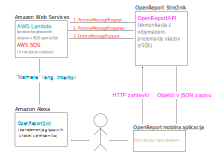
\includegraphics[width=11cm]{plan}
\end{center}
\caption{Visokonivojski načrt sistema}
\label{plan}
\end{figure}

\section{Uporabljene tehnologije in programska oprema}

\subsection{.NET}

.NET je razvojna platforma, razvita s strani Microsofta.
Obsega programske jezike, prevajalnike, orodja in knjižnice, ki omogočajo širok spekter primerov uporabnosti, hkrati pa se ohranja enovitost ozadne kode.

Tehnologije .NET ogrodja, ki sem jih uporabil v tej diplomski nalogi so:
\begin{itemize}
	\item .NET Core - odprtokodna platforma za razvoj spletnih storitev,
	\item Xamarin, ki je ogrodje za razvoj mobilnih aplikacij za najpogostejše mobilne operacijske sisteme (Android, iOS).
\end{itemize}

.NET sem izbral, saj je zelo dobro integriran z Amazonovim AWS API-jem in ker je dobro dokumentiran.

\subsection{Xamarin Forms}

Ogrodje Xamarin je odprtokodno orodje za razvoj mobilnih aplikacij, ki ga je razvil Microsoft. 
Je nadgradnja ogrodja .NET.

Z njim je mogoče pri preprostih aplikacijah deliti večino kode med različnimi operacijskimi sistemi. 
Za ozadno kodo se uporablja .NET (C\#), za front-end pa se uporablja XAML (Extensible Application Markup Language).

Xamarin sem izbral, saj imam z njim že predhodne izkušnje.

\subsection{Amazon Alexa}

Amazon Alexa je glasovni asistent, razvit s strani podjetja Amazon.
Za Amazon Alexo sem se odločil, saj ponuja enostavno možnost programiranja s ''Skill-i''.
Poleg tega je Alexo enostavno integrirati z drugimi Amazonovimi spletnimi storitvami, kot so AWS SQS.

\subsection{Alexa Skill}

Alexine osnovne funkcionalnosti lahko nadgradimo s funkcijami, ki se jim reče ''Skill''.
Da lahko ustvarimo in objavimo Skill rabimo račun Amazon razvijalca (\textit{ang. Amazon Developer}).


''Skill'' sestavljajo:
\begin{itemize}
	\item Invocation - fraza, ki Skill zažene,
	\item Intent - fraze, ki jih Skill razpozna kot funkcije,
	\item Endpoint - omrežni vir, kjer se nahaja ozadna koda Skill-a.
\end{itemize}

Ko Alexa zasliši Invocation ali katerega od Intentov, glasovni posnetek pošlje na Amazonov strežnik.
Ta s pomočjo strojnega učenja razpozna ukaze in pošlje ukaze na Endpoint.
To je lahko druga Amazonova storitev (npr. AWS Lambda), Microsoftov Azure strežnik ali naš lasten strežnik.
Ko Endpoint obdela zahtevo, se rezultat pošlje nazaj na Amazonov strežnik v obliki znakovnega niza.
Ta podatek se nato pošlje nazaj na uporabnikovo Alexo, ki prejeti znakovni niz izgovori.

\subsection{Amazon Web Services}

AWS je skupek oblačnih storitev, ki ga ponuja podjetje Amazon.
Ponuja integracijo s popularnimi programskimi jeziki in ogrodji, kot so Java, .NET, Python in Node.js preko AWS API storitve.
Pri tej diplomski nalogi sem se osredotočil na dva sistema iz skupka AWS.

\subsubsection{AWS SQS}

AWS SQS je sistem za pošiljanje tekstovnih sporočil med odjemalci preko Amazonovih strežnikov.
Za hranjenje sporočil je treba registrirati Queue ali vrsto. 
Ta je lahko navadna vrsta, kjer prejeta sporočila niso nujno urejena po času ustvarjanja, lahko pa je tipa FIFO.
Pri FIFO vrsti sporočila prejmemo v točno takšnem vrstnem redu, kot smo jih poslali.

To storitev bom uporabil za komunikacijo med Amazon Alexo in OpenReport strežnikom.

// ali še opišem SQS

\subsubsection{AWS Lambda}

// lepši prevod za hosting

Ozadno kodo za Alexa Skill sem objavil v platformo AWS Lambda.
To je storitev za gostovanje dogodkovno vodene ozadne kode.
Za to platformo sem se odločil zaradi dobre integracije z Alexa Skill Kit-om in razvojnim orodjem Visual Studio.

// ali še opišem Lambdo?

\section{Načrt delovanja strežnika}

// API endpointi

\section{Načrt in izdelava ,,Alexa Skilla''}

OpenReportSkill se bo začel izvajati z ''Invocation'' frazo ,,make a report note''.
Uporabnik lahko nato izbere med naslednjimi ukazi:
\begin{itemize}
	\item ''take note''
	\item ''create a text note''
	\item ''take a picture''
\end{itemize}
Alexa pošlje posnetek govora na Amazonov Alexa Server, kjer se zahteva obdela in primerja z nastavljenimi Intenti.
Frazi "note" ali "take note", na začetku narekovanega besedila, se ujemata s frazami za klic Intenta TakeNoteIntent.

Amazonov Alexa Server nato pošlje TakeNoteIntent in vsebino (na sliki \ref{skill} \{content\}) na nastavljen Endpoint.
Ta je v našem primeru gostovan na storitvi AWS Lambda.

Endpoint gosti ozadno kodo za obdelavo podatkov, ki jih Alexa Server pošlje.
V našem Endpointu se TakeNoteIntent obdela tako, da se \{content\} pošlje kot novo sporočilo v AWS SQS.
Ko je sporočilo poslano, Endpoint Alexa Serverju pošlje nazaj zahtevo Response.
Ta hrani niz, ki ga bo Alexa izgovorila uporabniku.
V našem primeru je to stavek "Noted!".

\begin{figure}[H]
\begin{center}
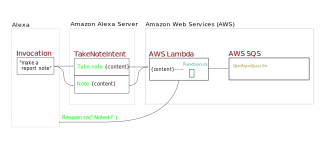
\includegraphics[width=11cm]{skill}
\end{center}
\caption{Načrt Alexa Skilla}
\label{skill}
\end{figure}


\section{Izdelava API}

\section{Izdelava delavca}

Delavec (ang. Worker Service) je storitev, ki se praviloma konstatno izvaja v ozadju.
V našem primeru se delavec uporablja za dobivanje sporočil iz AWS SQS sporočilne vrste in vstavljanje prejetih sporočil v podatkovno bazo.

Ustvaril sem ga tako, da sem v trenuten Solution dodal nov projekt tipa WorkerService.
Komponente takega projekta so predvsem razred Startup, ki se kliče prvi po zagonu programa in razred Program, v katerega pišemo poslovno logiko programa.

Pomemben del programiranja delavca je bil konfiguracija AWS storitev.
Zaradi varnosti, v projektne datoteke nisem neposredno vpisal vseh dostopnih podatkov za Amazonove spletne vire.
Najvarnejši način za dostopanje do teh podatkov je uporaba privzete AWS CLI lokacije za hranjenje dostopnih podatkov, ki se nahaja v domačem direktoriju uporabnika.
Natančneje, konfiguracijski datoteki se nahajata v mapi ''.aws'', poimenovani pa sta ''credentials'' in ''config''.

V datoteki appsettings.json, OpenReportWorkerService projekta, sem dodal sekcijo AWS.
Ta je kasneje uporabljena za avtentikacijo zahtev za delo s SQS sporočili.

Delavec deluje tako, da v while zanki, vsake 10 sekund, AWS SQS vrsto vpraša, ali je na voljo kakšno sporočilo, tako, da pošlje vrsti RecieveMessageRequest. 
Če je v prejetem RecieveMessageResponsu kakšno sporočilo, se za vsako sporočilo ustvari nov tip objekta Note.
Vsak se nato z API klicem nato vnese v podatkovno bazo.
Pripne se trenutno odprtemu projektu.

Ko je sporočilo vnešeno v podatkovni bazi, se lahko izbriše iz SQS vrste.
To dosežemo z DeleteMessageRequest-om.


\section{Postopek oblikovanja in načrtovanja mobilne aplikacije}

Mobilno aplikacijo sem se odločil razviti s tehnologijo Xamarin.Forms.
Razlogi za to so predvsem dobro poznavanje tehnologije in enostavna integracija z ostalimi tehnologijami iz .NET sklopa.
Prav tako se lahko ospredna XAML in ozadna C\# koda v veliki meri uporabita v drugih .NET rešitvah.

Postopek sem začel z premislekom o funkcionalnostih aplikacije.
Nato sem začel z skico pogledov na list papirja.
Ko sem prišel do željene oblike, sem s programom Inkscape narisal prototipe vseh pomembnejših pogledov.

\subsection{Pristop}
Pristop razvoja aplikacije, ki sem ga ubral se imenuje Model View View-Model (v nadaljevanju MVVM).
Pri tem pristopu aplikacijo razdelimo na tri dele.

\textbf{Model} je del, kjer definiramo elemente naše poslovne logike, prikaz podatkov, itd.

\textbf{View} je uporabniški vmesnik.

\textbf{ViewModel} pa se uporablja, da se poveže funkcije uporabniškega vmesnika in poslovne logike.

Rezultat upoštevanja tega pristopa je čista koda.
Model vsebuje le abstrakcijo naših podatkov in poslovno logiko.
Ti podatki se v ViewModelu pretvorijo v obliko, ki bo prikazana uporabniku.
View pa vsebuje izključno UI elemente in povezavo na ViewModel.

// slika mvvm

\subsection{Uvoz knjižnic in zunanjih virov v projekt}
Po dizajnu sem se lotil programiranja.
Najprej sem ustvaril prazen Xamarin projekt tipa Shell.
Najprej sem želel uvoziti funkcionalnosti, ki bi mi v prihodnjih fazah olajšale delo.
Prva taka stvar je bila uvoz razširitev Fody.
To je orodje, ki med prevajanjem MVVM aplikacije določene odseke C\# kode "vstavi" v preveden assembly.
S tem se ohrani ista funkcionalnost z veliko manj boilerplate kode.

// slika fody

Naslednja takšna funkcionalnost je bila uvoz fontov.
Za ikone nisem uporabil SVG ali PNG zbirk, ampak sem uporabil popularen font FontAwesome, ki ga nekoliko enostavneje uporabiti in uvoziti.

V projektu OpenReportShell.Android sem v Assets mapo dodal podmapo fonts.
V tej mapi se nahaja datoteka s FontAwesome Solid fontom.

Ta font sem uporabil tako, da sem v osnovnem projektu dodal Resource v datoteki App.xaml.

// slika resource

\subsection{Povezava na strežnik in razred Startup.cs}

Za povezavo na strežnik sem želel v projektu imeti eno instanco statičnega razreda.
Ta razred (OpenReportCloudCommunicationService) vsebuje metode, namenjene komunikaciji z API-jem.

Registriral sem ga po metodi DependencyInjection.
To sem dosegel tako, da sem v projekt dodal razred Startup.cs.
V tem razredu sem registriral razred ServiceProvider, s katerim bom lahko dostopal do registriranih razredov drugod po aplikaciji.

V ServiceProvider sem dodal dva razreda.
Prvi je HttpClient, ki sem ga uporabil za pošiljanje HTTP sporočil na strežnik, drugi pa je OpenReportServerCommunicationService, ki je bil uporabljen za formiranje HTTP sporočil.

// slika ConfigureServices

// slika OpenReportServerCommunicationService

\subsection{DashboardPage}

Na strani DashboardPage se uporabniku prikaže seznam odprtih projektov.
Ko uporabnik klikne na željeni projekt, ga preusmeri na stran ProjectPage, kjer ga lahko ureja.
Če nanj pridrži, se mu pokažejo dodatne opcije, kot so izbris in ahriviranje.

// slika DashboardPage

\subsection{ProjectPage}

Najpomembnejši del aplikacije je urejanje zapiskov.
To lahko uporabnik dela, 

\section{Evalvacija funkcionalnosti}

\chapter{Možnosti nadaljnega razvoja}
\chapter{Zaključek}

% \section{Formati slik}
% 
% Bitne slike, vektorske slike, kakršnekoli slike, z \LaTeX{}om lahko vključimo vse.
% Slika~\ref{pic1} je v {\tt .pdf} formatu.
% \begin{figure}[h]
% \begin{center}
% \includegraphics[width=0.6\textwidth]{pic1.pdf}
% \end{center}
% \caption{Herschelov graf, vektorska grafika.}
% \label{pic1}
% \end{figure}
% Pa res lahko vključimo slike katerihkoli formatov? 
% Žal ne. 
% Programski paket \LaTeX\ lahko uporabljamo v več dialektih. 
% Ukaz {\tt latex} ne mara vključenih slik v formatu Portable Document Format {\tt .pdf}, ukaz {\tt pdflatex} pa ne prebavi slik v Encapsulated Postscript Formatu {\tt .eps}.
% Strnjeno je vključevanje različnih vrst slikovnih datotek prikazano v tabeli~\ref{tbl:1}.


\newpage %dodaj po potrebi, da bo številka strani za Literaturo v Kazalu pravilna!
\ \\
\clearpage
\addcontentsline{toc}{chapter}{Literatura}

%\printbibliography

\end{document}

